%Listing definition for XML

\definecolor{gray}{rgb}{0.4,0.4,0.4}
\definecolor{darkblue}{rgb}{0.0,0.0,0.6}
\definecolor{cyan}{rgb}{0.0,0.6,0.6}

\lstset{
  basicstyle=\ttfamily,
  columns=fullflexible,
  showstringspaces=false,
  commentstyle=\color{gray}\upshape
}

\lstdefinelanguage{XML}
{
  morestring=[b]",
  morestring=[s]{>}{<},
  morecomment=[s]{<?}{?>},
  stringstyle=\color{black},
  identifierstyle=\color{darkblue},
  keywordstyle=\color{cyan},
  morekeywords={}% list your attributes here
}

%%%%%%%%%%%%%%%%%%%%%%%%%%%%%%%%%%%%%%%%%%%%%%%%%%%%%%%%%%%%%%%%%%%%%%%%%%%%%

%Listing definition for Java
\definecolor{javared}{rgb}{0.6,0,0} % for strings
\definecolor{javagreen}{rgb}{0.25,0.5,0.35} % comments
\definecolor{javapurple}{rgb}{0.5,0,0.35} % keywords
\definecolor{javadocblue}{rgb}{0.25,0.35,0.75} % javadoc

\lstset{prebreak=\raisebox{0ex}[0ex][0ex]
        {\ensuremath{\rhookswarrow}}}
\lstset{postbreak=\raisebox{0ex}[0ex][0ex]
        {\ensuremath{\rcurvearrowse\space}}}
\lstset{breaklines=true, breakatwhitespace=true}
\lstset{numbers=left, numberstyle=\scriptsize}
 
\lstset{language=Java,
basicstyle=\ttfamily,
keywordstyle=\color{javapurple}\bfseries,
stringstyle=\color{javared},
commentstyle=\color{javagreen},
morecomment=[s][\color{javadocblue}]{/**}{*/},
numbers=left,
numberstyle=\tiny\color{black},
stepnumber=2,
numbersep=10pt,
tabsize=4,
showspaces=false,
showstringspaces=false
}

%%%%%%%%%%%%%%%%%%%%%%%%%%%%%%%%%%%%%%%%%%%%%%%%%%%%%%%%%%%%%%%%%%%%%%%%%%%%%%%%%

\chapter{Implementation}

\section{Technologies used}

As it has been explained previously, the two modules developed as part of the work for this thesis have been designed to be integrated with the Hummingbird project. To do so, Java\cite{Java} has been chosen as the main programming language, as it is the language used for the development of Hummingbird. In the same way, Apache Camel\cite{Camel} and ActiveMQ \cite{AMQ} are used for the communication with the rest of the modules. XStream\cite{XStream} has been chosen as the library used to parse the XML\cite{XML} files used to specify the scientific information.

The final piece of technology used is BeanShell\citep{BSH}, a Java-like scripting language and interpreter which runs in the Java Runtime Environment. The calibration module has been designed to be generic, adaptable to every mission. Also, the goal was to make the calibration information input easy for the scientists, meaning this no need to any difficult Java programming, compilation and so on. BeanShell integrates with the Java code and allows to run those scripts at runtime.

\section{Implementation of the calibration module}

For the sake of clarity, the approach to the explanation will be in small pieces. However, before jumping onto every small piece, it is interesting to look at the package organization of the module.

The software is divided into several Java packages being those the following:
\begin{itemize}
\item \textbf{eu.estcube.calibration}: contains the Apache Camel integration. It also contains the main class of the module.
\item \textbf{eu.estcube.calibration.calibrate}: contains the implementation of the calibrator.
\item \textbf{eu.estcube.calibration.constants}: contains several constants used throughout the module.
\item \textbf{eu.estcube.calibration.domain}: contains the data structures used to represent the calibration information and the calibration units.
\item \textbf{eu.estcube.calibration.processors}: contains the main algorithm for receiving, calibrating and sending the parameters back. Also, the interface implemented by the calibrator can be found here.
\item \textbf{eu.estcube.calibration.utils}: contains additional utilities. In this case, the tools to manage finding and reading files.
\item \textbf{eu.estcube.calibration.xmlparser}: contains the tools to parse the information contained in XML format into data which can be used in the module.
\end{itemize}

\subsection{Camel Integration}

The integration with Camel is a crucial part of the module since it is where it will take the parameters from. There are several classes related to this, the class diagram of this part can be seen in Figure \ref{f5.1}. 

\begin{figure}[H]
\centerline{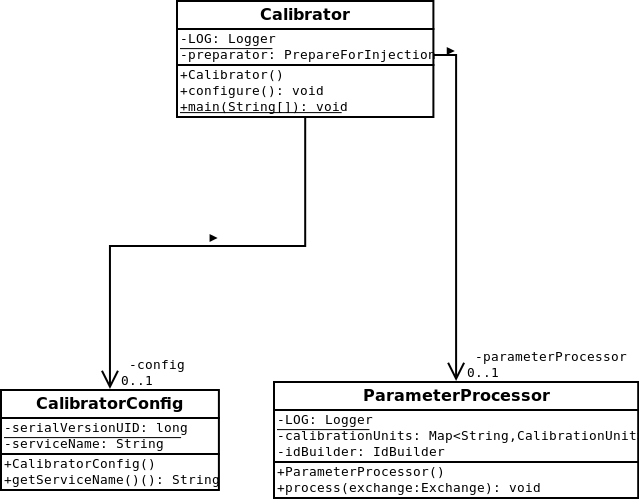
\includegraphics[width=0.75\textwidth]{images/CalibratorCamelClassDiagram.png}}
\caption{Class diagram of the Camel integration}
\label{f5.1}
\end{figure}

Amongst the three classes represented in Figure \ref{f5.1} it is important to highlight two of them: \emph{Calibrator} and \emph{ParameterProcessor}.

\emph{Calibrator} is the main class of the module. As it is shown in the class diagram there are two methods, the \textbf{main} method, where everything starts and the \textbf{configure} method. The latter is where the integration with Camel happens, what configures where to get the messages from, what to do with them and where to send them afterwards. In addition, \emph{Hummingbird} utilizes a heartbeat system to check if the modules are working correctly, this is also carried on here. Table \ref{Table5.1} contains a snippet of the code.

\begin{table}[h]
\lstset{language=Java}
\begin{lstlisting}

    @Override
    public void configure() throws Exception {

        // @formatter:off
        from(StandardEndpoints.MONITORING)
            .filter(header(StandardArguments.CLASS)
            .isEqualTo(Parameter.class.getSimpleName()))
            .process(parameterProcessor)
            .split(body())
            .process(preparator)
            .to(StandardEndpoints.MONITORING);
        
        BusinessCard card = new BusinessCard(config.getServiceId(), config.getServiceName());
        card.setPeriod(config.getHeartBeatInterval());
        card.setDescription(String.format("Calibrator; version: %s", config.getServiceVersion()));
        from("timer://heartbeat?fixedRate=true&period=" + config.getHeartBeatInterval())
            .bean(card, "touch")
            .process(preparator)
            .to(StandardEndpoints.MONITORING);
        // @formatter:on

    }



\end{lstlisting}
\caption{Camel integration Java code for the calibrator}
\label{Table5.1}
\end{table}
\_cal
\pagebreak
Focusing on the part where the module receives and sends the parameters we can see that:

\begin{itemize}
\item Where it gets the messages from --> \emph{from(StandardEndpoints.MONITORING)}
\item It only gets messages containing parameters -->  \emph{.filter(header(StandardArguments.CLASS)}
            \emph{.isEqualTo(Parameter.class.getSimpleName()))}
\item What to do with the received message --> \emph{.process(parameterProcessor)}
\item Since the result of the processed message is a list and it is necessary to send the parameters one by one, that result must be split. --> \emph{.split(body())}
\item Send it back to the messaging service --> \emph{.process(preparator)}\linebreak
            \emph{.to(StandardEndpoints.MONITORING);}

\end{itemize}


The second part - from line 14 and below - contains the heartbeat system.


\emph{ParameterProcessor} contains the following:
\begin{itemize}
\item Part of the Camel integration.
\item Code to load the calibration information from the configuration files.
\item Algorithm to process the received parameters.
\end{itemize}

The code corresponding to the Camel integration is shown in table \ref{Table5.2}. The other two parts will be explained in the following subsections.

\begin{table}[h]
\lstset{language=Java}
\begin{lstlisting}

    /** @{inheritDoc . */
    @Override
    public void process(Exchange exchange) throws Exception {

        Message in = exchange.getIn();
        Message out = exchange.getOut();
        out.copyFrom(in);

    		//The main algorithm would be placed here    

        out.setBody(calibratedParameters);

	}


\end{lstlisting}
\caption{Java code showing the Camel integration of \emph{ParameterProcessor} }
\label{Table5.2}
\end{table}

\subsection{Loading the calibration information}

The first action point when the module is initiated is loading the calibration information. This will read the information from the configuration files written by the specialists and will create a series of calibration units which will later be used to calibrate the incoming parameters.

Figure \ref{f5.2} shows the different classes involved in this process. They can be organised as follows:
\begin{itemize}
\item Main class: \emph{ParameterProcessor}
\item Data structures:
	\begin{itemize}
		\item \emph{CalibrationUnit}
		\item \emph{InfoContainer}
	\end{itemize}
\item Utils:
	\begin{itemize}
		\item \emph{InitCalibrationUnits}
		\item \emph{InitCalibrators}
		\item \emph{FileManager}
	\end{itemize}
\item Parser:
	\begin{itemize}
		\item \emph{Parser}
		\item \emph{HashMapConverter}
	\end{itemize}
\end{itemize}


\begin{figure}[H]
\centerline{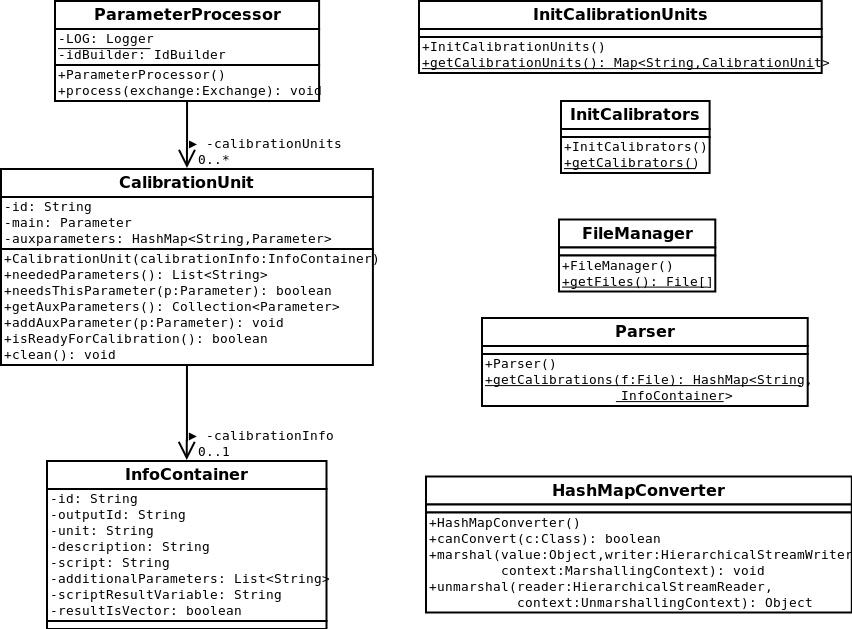
\includegraphics[width=1.3\textwidth]{images/LoadInfoClassDiagram.png}}
\caption{Diagram of the classes involved in loading the calibration information onto the system.}
\label{f5.2}
\end{figure}




The best way to see how these classes interact with each other is by looking at its sequence diagram (Figure \ref{f5.3}). The main class is \emph{ParameterProcessor}, where the calibration information will be stored in the form of a \emph{HashMap} of calibration units. The reason for choosing a this data structure is its efficiency, as it provides constant-time performance for the input and retrieval of information\cite{HashMap}. The process begins by \emph{ParameterProcessor} asking \emph{InitCalibrationUnits} to initialize them. To do so the calibration units need the calibration information (calibrators), which is initialized  by \emph{InitCalibrators}. \emph{InitCalibrators} is the class which manages the access to information in the files; first it finds the corresponding XML files to later parse each of them, creating the calibrators. With this calibrators, \emph{InitCalibrationUnits} creates them, and then returns them to the main class where they are ready to receive the incoming parameters.

There is one class present in the class diagram in Figure \ref{f5.2} which is not present in Figure \ref{f5.3}: \emph{HashMapConverter}. This is because this class is managed by \emph{XStream}, the external library used to simplify XML access and parsing. 


\begin{figure}[H]
\centerline{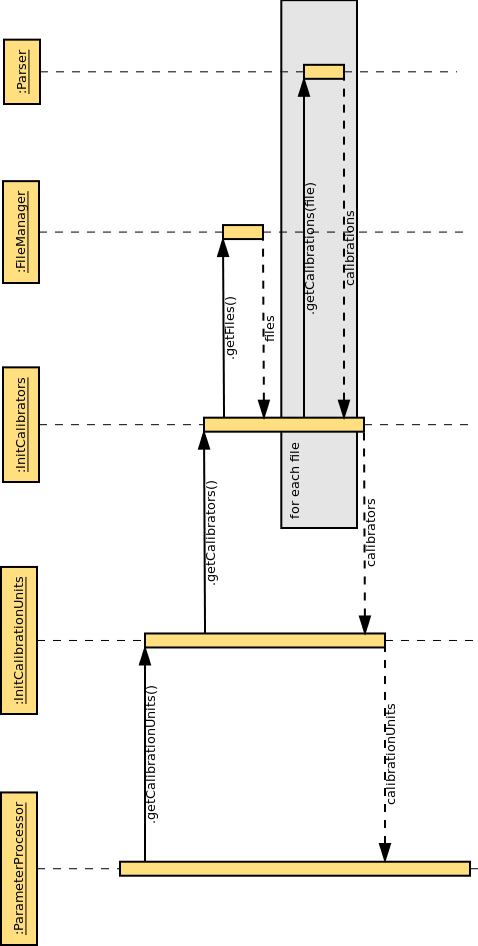
\includegraphics[width=0.75\textwidth]{images/InitCalibrationUnitsSequence.png}}
\caption{Sequence diagram which represents the interactions between the different classes present when loading the calibration information.}
\label{f5.3}
\end{figure}


The data structure created to represent the calibration information is \emph{InfoContainer} and it is formed by these components:

\begin{itemize}

	\item \textbf{id}
		\begin{itemize}
			\item Type: String
			\item Content: name of the parameter to be calibrated
		\end{itemize}
	\item \textbf{outputId}
		\begin{itemize}
			\item Type:String
			\item Content: name of the engineering parameter
		\end{itemize}
	\item \textbf{unit}
		\begin{itemize}
			\item Type: String
			\item Content: unit in which the calibrated value is represented
		\end{itemize}
	\item \textbf{Description}
		\begin{itemize}
			\item Type:String
			\item Content:description of the parameter
		\end{itemize}
	
	\item \textbf{additionalParameters}
		\begin{itemize}
			\item Type: List of Strings
			\item Content: List with the names of any extra parameters needed for the calibration
		\end{itemize}
	\item \textbf{resultIsVector}
		\begin{itemize}
			\item Type: boolean
			\item Content: $true$ if the result of the calibration is a vector, $false$ if the result of the calibration is an individual value 
		\end{itemize}
	\item \textbf{scriptResultVariable}
		\begin{itemize}
			\item Type: String
			\item Content: name of the variable which will contain the result in the script
		\end{itemize}
	\item \textbf{script}\_cal
		\begin{itemize}
			\item Type: String
			\item Content: calibration script
		\end{itemize}						
		
\end{itemize}

This data structure is later stored within another data structure, \emph{CalibrationUnit}. The reason for using this second data structure is the way parameters are received from Camel, one by one. If all the calibrations were just simple one-parameter calibrations that would not be necessary. However, some parameters might need information from others to be calibrated, thus, they need to be sent as a whole unit to the method to the method which will generated the engineering values. \emph{CalibrationUnit} is formed by the following components:

\begin{itemize}
\item Attributes:
	\begin{itemize}
		\item \textbf{id}
			\begin{itemize}
				\item Type: String
				\item Content: name of the parameter to be calibrated
			\end{itemize}
		\item \textbf{main}
			\begin{itemize}
				\item Type: Parameter
				\item Content: parameter which will be calibrated
			\end{itemize}				
		\item \textbf{auxParameters}
			\begin{itemize}
				\item Type: HashMap of Parameters
				\item Content: extra parameters needed to calibrate the main one
			\end{itemize}												
		
	\end{itemize}
	
	\item Amongst others, \emph{CalibrationUnit} can perform the following actions:
	\begin{itemize}
		\item \textbf{neededParameters}: returns the parameters listed as necessary for the calibration
		\item \textbf{needsThisParameter}: checks whether or not a particular parameter is needed for the current calibration unit
		\item \textbf{addAuxParameter}: adds an extra parameter when needed
		\item \textbf{isReadyForCalibration}: checks that all the needed parameters are in place. Only when this check returns true the calibration unit is sent to the calibrator.
		\item \textbf{clean}: once the calibration unit has been sent to the calibrator, it is cleaned so it can be used for the next time that parameters are received. This means emptying the main and auxiliary parameters.
	\end{itemize}

\end{itemize}


\subsection{Calibration}
The calibration process can be divided in two parts. The first one is managing the parameters that arrive from other modules, prepare the calibration units and send back the results. The second is the actual calibration. 

Figure \ref{f5.4} represents the class diagram of this part of the software. There are three classes which have been seen in previous sections ---\emph{ParameterProcessor}, \emph{CalibrationUnit} and \emph{InfoContainer}--- and two new ones which are:
\begin{itemize}
\item \emph{ParameterCalibrator}: Interface representing the method that the calibrator must contain.
\item \emph{Calibrate}: Implementation of the previous interface, where the actual calibration is performed. This class is generic class. Its generic type \emph{T} extends from Java Number, which means any the Java Number subtypes can be used when instantiating it. Currently is in the form of a Double, but it can be easily modified if ever needed.
\end{itemize}


\begin{figure}[H]
\centerline{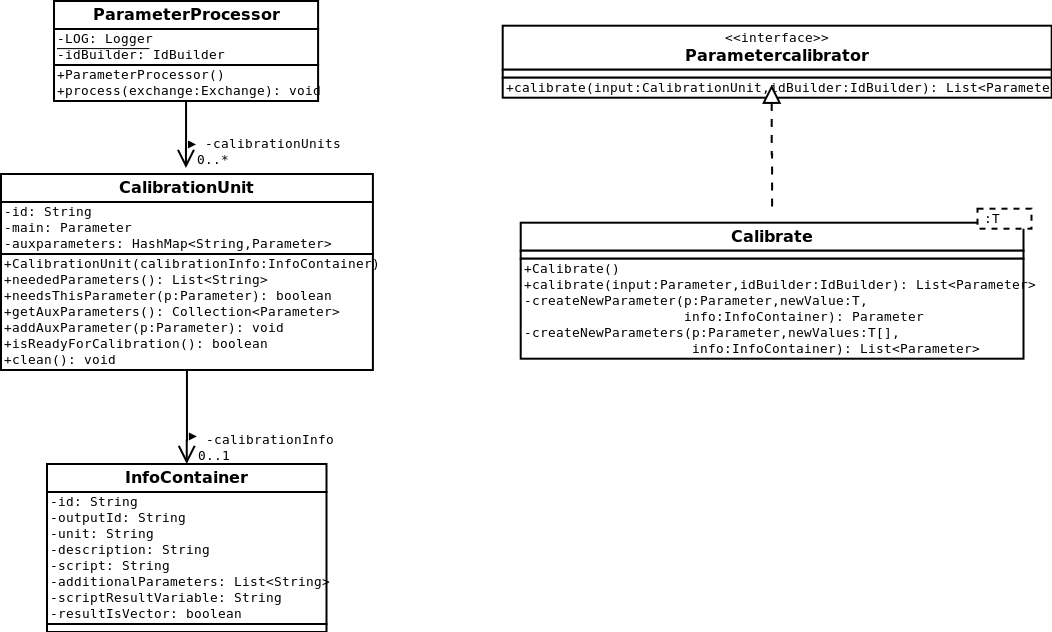
\includegraphics[width=1.2\textwidth]{images/CalibrationClassDiagram.png}}
\caption{Diagram representing the classes involved in the calibration process.}
\label{f5.4}
\end{figure}

Figure \ref{f5.5} is a flow chart representing the algorithm used to manage the received parameters, in combination with the sequence diagram of Figure \ref{f5.6} they show what the steps in the algorithm are and which parts of the software performs then. As it was previously stated, the main class is \emph{ParameterProcessor}, where the calibration units have already been created. When a parameter is received, if its corresponding calibration unit is available it is included as its main part (if it is not present, the process ends with an error log message). Afterwards, the algorithm goes through every calibration unit doing the following:
\begin{enumerate}
\item Check if the parameter is needed for the calibration unit.
\item If 1 is true, add the parameter as an auxiliary parameter for the calibration.
\item Check if the calibration unit is ready for calibration.
\item If 3 is true, calibrate and save the results in a list. Finally, clean the calibration unit.
\end{enumerate}

After the whole process is completed the results are sent back to Camel so make them available for the rest of the system.

\begin{figure}[H]
\centerline{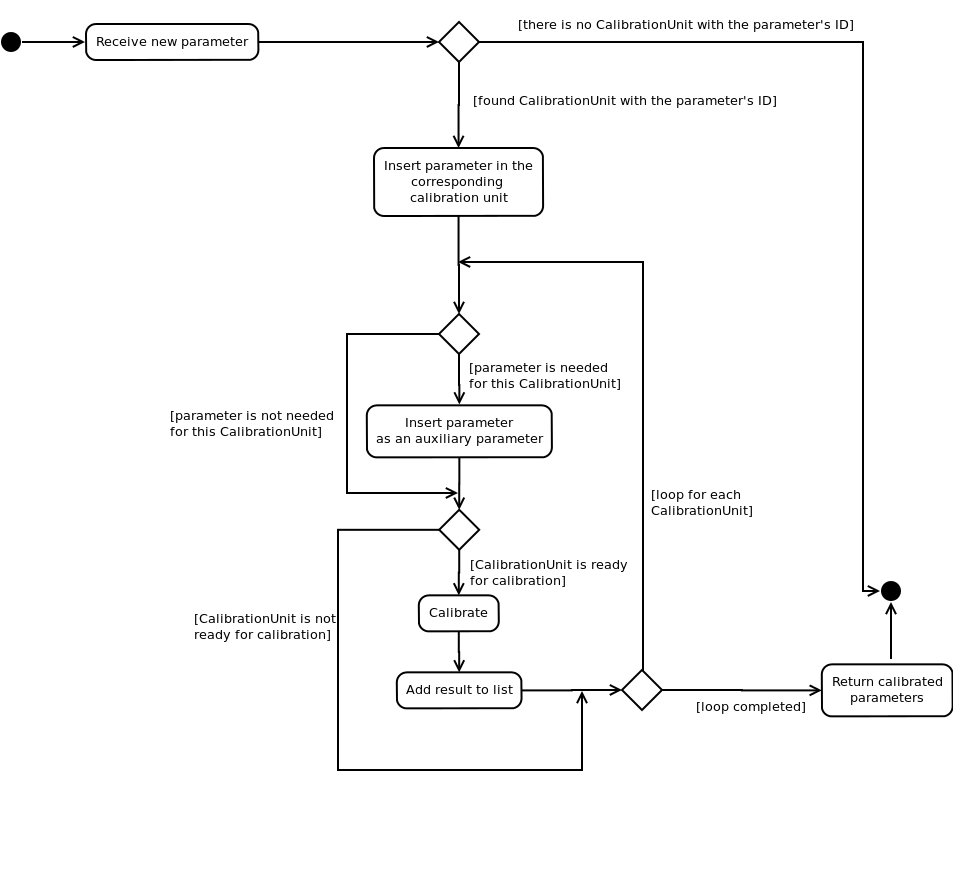
\includegraphics[width=1.2\textwidth]{images/ReceiveParameterAndCalibrateFlowChart.png}}
\caption{Flow chart of the algorithm to manage incoming parameters in the calibration module.}
\label{f5.5}
\end{figure}


\begin{figure}[H]
\centerline{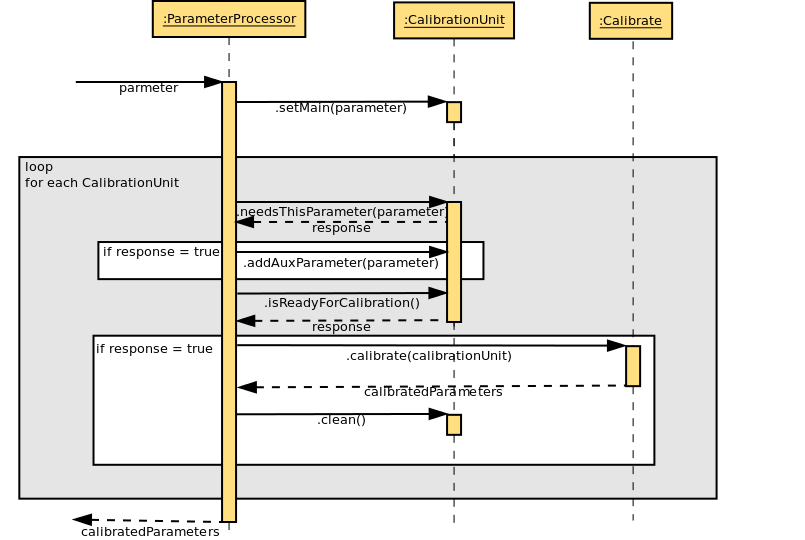
\includegraphics[width=1.2\textwidth]{images/ReceiveParameterAndCalibrateSequence.png}}
\caption{Sequence diagram describing the interactions between the different classes when managing incoming parameters in the calibration module.}
\label{f5.6}
\end{figure}


The part of evaluating the raw parameters using the calibration script is left in the hands of \emph{BeanShell}. The way to evaluate a script with this library is very simple as it can be seen in Table \ref{Table5.2}. 


\begin{table}[h]
\lstset{language=Java}
\begin{lstlisting}
  Interpreter interpreter = new Interpreter();
  interpreter.eval(calibrationScript);
\end{lstlisting}
\caption{Java code used to evaluate a script with \emph{BeanShell}.}
\label{Table5.2}
\end{table}


Table \ref{Table5.4} shows the way information is retrieved from the interpreter and how the parameters with the engineering values are created. The actions to be taken change depending on the result being a vector or not.

\begin{table}[h]
\lstset{language=Java}
\begin{lstlisting}
  if (input.getCalibrationInfo().isResultIsVector()) {

            T[] calibratedValues = (T[]) interpreter.get(input.getCalibrationInfo()
                .getScriptResultVariable());
            output.addAll(createNewParameters(input.getMain(), calibratedValues, input.getCalibrationInfo()));

        } else {

            T calibratedValue = (T) interpreter.get(input.getCalibrationInfo()
              .getScriptResultVariable());
            output.add(createNewParameter(input.getMain(), calibratedValue,
                    input.getCalibrationInfo()););

        }
\end{lstlisting}
\caption{Java code used to retrieve the information from the interpreter and generate the new parameters.}
\label{Table5.4}
\end{table}


\section{Implementation of the limit checking module}

This module also has a very similar structure to the calibration one. The explanation will once again be divided in small pieces, some of them very similar to the ones already explained for the calibration module. The overall package structure of the module is the following:

\begin{itemize}
\item \textbf{eu.estcube.limitchecking}: contains the Apache Camel integration. It also contains the main class of the module.
\item \textbf{eu.estcube.limitchecking.checklimits}: contains the classes where the limit checking is performed.
\item \textbf{eu.estcube.limitchecking.constants}: contains several constants which are used throughout the module.
\item \textbf{eu.estcube.limitchecking.domain}: contains the data structure used to represent the limits information.
\item \textbf{eu.estcube.limitchecking.processors}: contains the main algorithm for receiving, checking the limits and sending the results back. Also, the interface implemented by the limit checker can be found here.
\item \textbf{eu.estcube.limitchecking.utils}: contains additional utilities. In this case, the tools to manage finding and reading files.
\item \textbf{eu.estcube.limitchecking.xmlparser}: contains the tools to parse the information contained in XML format into data which can be used in the module.
\end{itemize}
\subsection{Camel integration}

The integration with camel is done in the exact same way as in the calibration module. Figure \ref{f5.7} contains a diagram of the classes involved in this process. The classes change their name (\emph{Calibrator} to \emph{LimitChecking} and \emph{CalibratorConfig} to \emph{LimitCheckingConfig}) and a the \textbf{split} option is removed (compare Tables \ref{Table5.1} and\ref{Table5.5}, as there is no need to split results received from \emph{ParameterProcessor}. There are also some minor changes in the latter, but those are related to the limit checking and not to the Camel integration. For more information please see the correspondent section in the calibration module.

\begin{figure}[H]
\centerline{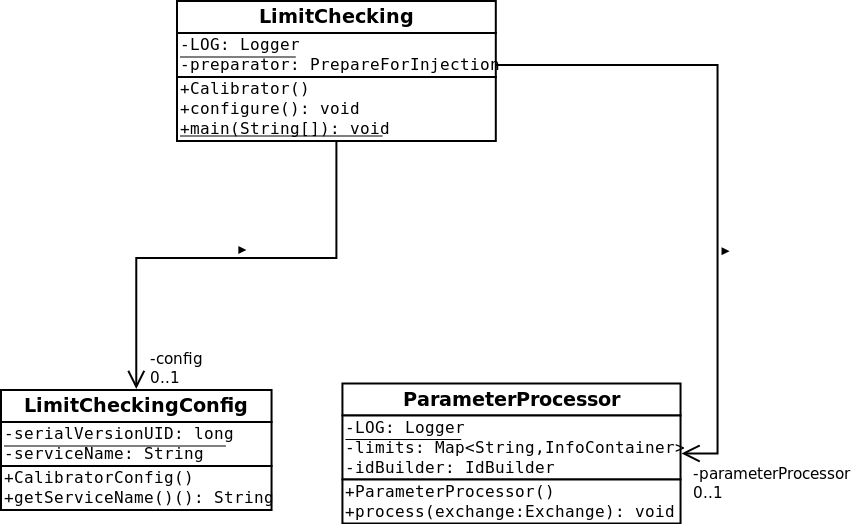
\includegraphics[width=0.75\textwidth]{images/LimitCheckingCamelClassDiagram.png}}
\caption{Class diagram of the Camel integration}
\label{f5.7}
\end{figure}
\pagebreak
\begin{table}[H]
\lstset{language=Java}
\begin{lstlisting}

    @Override
    public void configure() throws Exception {

        // @formatter:off
        from(StandardEndpoints.MONITORING)
            .filter(header(StandardArguments.CLASS)
            .isEqualTo(Parameter.class.getSimpleName()))
            .process(parameterProcessor)
            .process(preparator)
            .to(StandardEndpoints.MONITORING);
        
        BusinessCard card = new BusinessCard(config.getServiceId(), config.getServiceName());
        card.setPeriod(config.getHeartBeatInterval());
        card.setDescription(String.format("Calibrator; version: %s", config.getServiceVersion()));
        from("timer://heartbeat?fixedRate=true&period=" + config.getHeartBeatInterval())
            .bean(card, "touch")
            .process(preparator)
            .to(StandardEndpoints.MONITORING);
        // @formatter:on

    }



\end{lstlisting}
\caption{Camel integration Java code for the limit checker.}
\label{Table5.5}
\end{table}

\pagebreak

\subsection{Loading the limits information}
This is also done in the same way as it is performed in the calibration module. The first thing done when the module is initiated is loading the limits information. This means reading the information from the configuration files and creating the limits which will be later used to compare against the incoming parameters.
Figure \ref{f5.8} shows the different classes involved in this process. They can be organised as follows:
\begin{itemize}
\item Main class: \emph{ParameterProcessor}
\item Data structure: \emph{InfoContainer}
\item Utils:
	\begin{itemize}
		\item \emph{InitLimits}
		\item \emph{FileManager}
	\end{itemize}
\item Parser:
	\begin{itemize}
		\item \emph{Parser}
		\item \emph{HashMapConverter}
	\end{itemize}
\end{itemize}

\begin{figure}[H]
\centerline{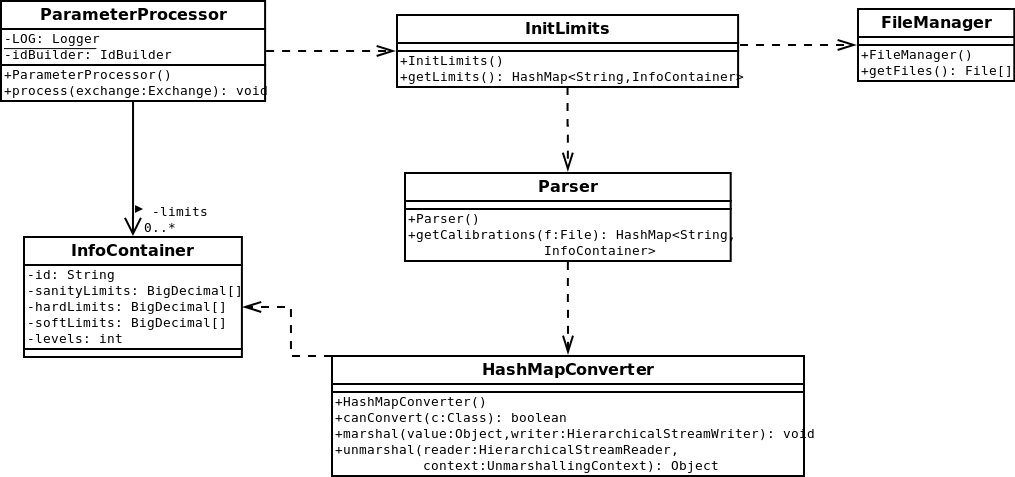
\includegraphics[width=1.3\textwidth]{images/LoadLimitsClassDiagram.png}}
\caption{Diagram of the classes involved in loading the limits information onto the system.}
\label{f5.8}
\end{figure}
\pagebreak

Figure \ref{f5.9} shows the sequence of message exchanges between the different classes involved in this process. Just as in the calibration module, the process begins at \emph{ParameterProcessor} and the limits will also be stored in a \emph{HashMap}, each entry corresponding to a different parameter. \emph{InitLimits} is the class in charge of populating that HashMap and to do so it follows the exact same process as the one explained for the calibration module. 



\begin{figure}[H]
\centerline{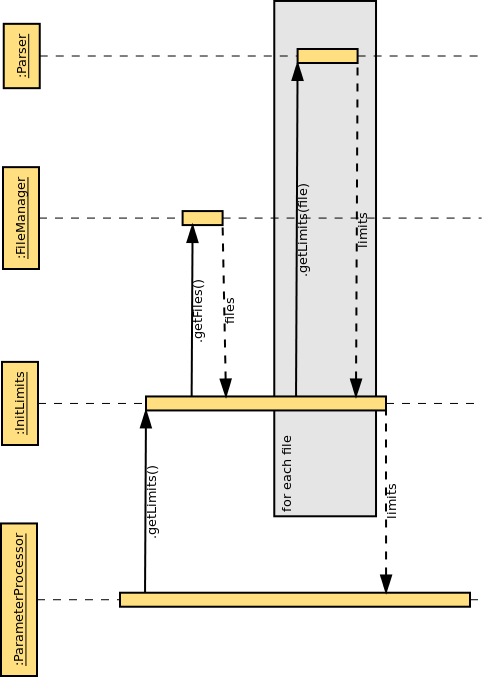
\includegraphics[width=0.75\textwidth]{images/InitLimitsSequence.png}}
\caption{Sequence diagram which represents the interactions between the different classes present when loading the limits information.}
\label{f5.9}
\end{figure}
\pagebreak
The data structure used to represent the limits information is, as it was in the previous module, \emph{InfoContainer}. However, its inner structure differs to the one which was previously used:

\begin{itemize}
	\item \textbf{id}
		\begin{itemize}
			\item Type: String
			\item Content: name of the corresponding parameter
		\end{itemize}
	\item \textbf{sanityLimits}
		\begin{itemize}
			\item Type: Array of $BigDecimal$\cite{BigDecimal}. This number format has been chosen as it provides high precision, avoiding rounding errors from other types, such as $double$.
			\item Content: lower limit in the first position and and upper limit in the second. This limits are optional, if enabled, four regions are available (discard, error, warning and OK). Any values below the lower or above the upper limits are discarded.
		\end{itemize}
	\item \textbf{hardLimits}
		\begin{itemize}
			\item Type: Array of $BigDecimal$.
			\item Content: lower limit in the first position and upper limit in the second. Anything between this limits and the soft limits is in the warning zone. Anything below the lower or above the upper limits is erroneous.
		\end{itemize}
	\item \textbf{softLimits}
		\begin{itemize}
			\item Type: Array of $BigDecimal$.
			\item Content: lower limit in the first position and upper limit in the second. Anything within these limits is in the OK region.
		\end{itemize}
		
	\item \textbf{levels}
		\begin{itemize}
			\item Type: Integer
			\item Content: automatically generated. Its value is 4 if sanity limits are available or 3 if they are not.
		\end{itemize}
\end{itemize}
\pagebreak

\subsection{Limit checking}

The process to check the limits of a parameter can also be divided in two, in the same way as the calibration module.

The different classes involved in this  part are represented in the class diagram in Figure \ref{f5.10}. There are three new classes used:

\begin{itemize}
	\item \emph{CheckLimits}: abstract class which implements the common methods used independently of the sanity limits being enabled or not. \textbf{isInErrorRegion(...)} and \textbf{checkLimits(...)} change depending on that fact, so they are implemented by its subclasses.
	\item \emph{CheckLimitsThreeLevels}: subclass of \emph{CheckLimits}. Used when the sanity limits are disabled.
	\item \emph{CheckLimitsFourLevels}: subclass of \emph{CheckLimits}. Used when the sanity limits are enabled. 
\end{itemize}


\begin{figure}[H]
\centerline{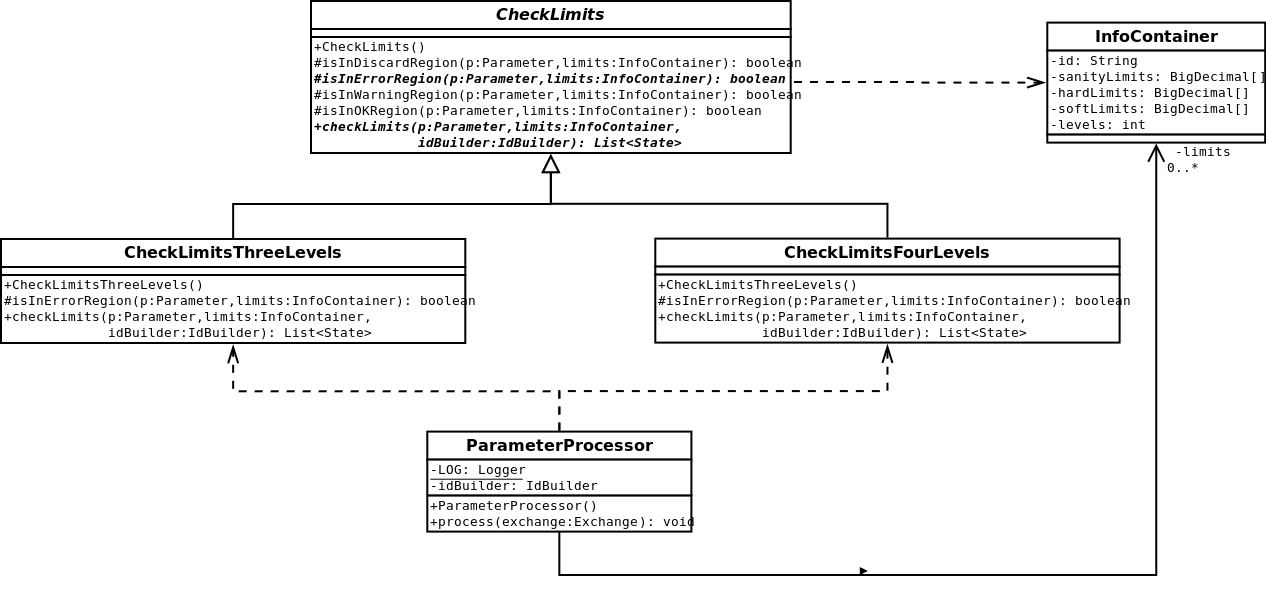
\includegraphics[width=1.4\textwidth]{images/CheckLimitsClassDiagram.png}}
\caption{Diagram representing the classes involved in the limit checking process.}
\label{f5.10}
\end{figure}

The flow of the process can be seen in Figure \ref{f5.11} whereas Figure \ref{5.12} shows the sequence diagram with the messages between the classes. For the sake of clarity, \emph{CheckLimits} should be interpreted as \emph{CheckLimitsThreeLevels} or \emph{CheckLimitsFourLevels}, depending on the case. This algorithm is much simpler than the one used for the calibration; the main class is \emph{ParameterProcessor}, where the limits information is stored. When a parameter is received, the first thing the algorithm does is check for its limits. If they are not present the process will end with and log error message. If everything goes correctly, the parameter will be sent to either \emph{CheckLimitsThreeLevels} or \emph{CheckLimitsFourLevels}.
Per request from the \emph{Hummingbird} architect, the result is returned as a list of $State$. The list has for elements, being:
\begin{itemize}
\item Discard region (if the sanity limits are disabled this state is automatically set to false).
\item Error region
\item Warning region
\item OK region
\end{itemize}

\begin{figure}[H]
\centerline{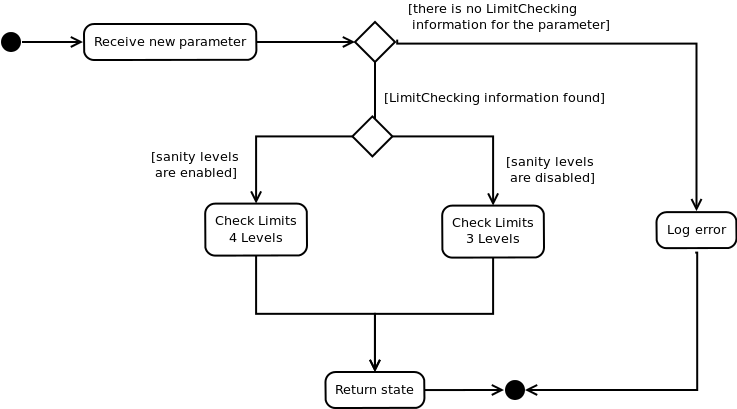
\includegraphics[width=1\textwidth]{images/LimitCheckingFlowChart.png}}
\caption{Diagram representing the classes involved in the limit checking process.}
\label{f5.11}
\end{figure}


\begin{figure}[H]
\centerline{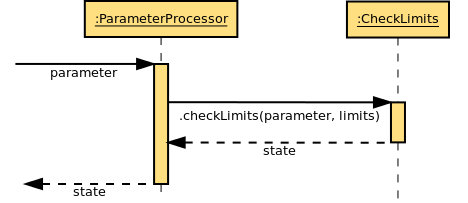
\includegraphics[width=0.75\textwidth]{images/CheckLimitsSequence.png}}
\caption{Diagram representing the classes involved in the limit checking process.}
\label{f5.12}
\end{figure}






\section{User manual}
\subsection{Calibration module}
This short user manual covers the use of the calibration module. The process is fully automated, so the user only needs to configure the pertinent XML file containing the information related to all the parameters which need to be calibrated.

There should be one file per subsystem. This way, the person who is making the changes will not have to be worried about modifying some other parts they do not understand. It is advisable that each file is called as the corresponding subsystem.


The location of the folder where the XML files are stored is fully configurable by a system property. It can be set like this: \textbf{-Dpath="/path/to/the/folder"}.
\pagebreak
\subsubsection{Structure of the XML file}

The XML file follows the format of Table \ref{Table5.6}
\begin{table}[H]
\lstset{language=XML}
\begin{lstlisting}

<calibration>
	<entry>
		<id></id>
		<description></description>
		<outputId></outputId>
		<unit></unit>
		<scriptInfo>
			<isVector></isVector>
			<resultVariable></resultVariable>
			<auxParameters></auxParameters>
			<script></script>
		</scriptInfo>
	</entry>
</calibration>
\end{lstlisting}
\caption{Structure of the XML file used to configure the calibrators.}
\label{Table5.6}
\end{table}

\begin{itemize}
\item \textbf{id}: name of the parameter to calibrate.
\item \textbf{Description}: description of the parameter.
\item \textbf{outputId}: name of the parameter generated after the calibration. If left blank, it will be the same as \textbf{id}.
\item \textbf{unit}: Units in which the value is represented.
\item \textbf{isVector}: \textbf{true} if the result of the calibration is a vector with several values (which generates several new parameters) or \textbf{false} if the calibration returns a single value.
\item \textbf{resultVariable}: variable in the script in which the result will be stored.
\item \textbf{auxParameters}: if the are extra parameters needed for the calibration process it is necessary to list them here separated by commas (','). Please note that if the extra parameters also needs to be calibrated the parameters needed for its calibration also must be included here in addition to the original one.
\item \textbf{script}: script to generate the calibrated value. Please note that if extra parameters are needed, their calibration script must be included here, not the parameter name. 
\end{itemize}

\subsubsection{Example of simple calibration}

\begin{table}[H]
\lstset{language=XML}
\begin{lstlisting}

<calibration>
	<entry>
		<id>parameterA</id>
		<description>Example of parameter for
		 simple calibration</description>
		<outputId>generatedA</outputId> 
		<unit>E</unit>
		<scriptInfo>
			<isVector>false</isVector>
			<resultVariable>result</resultVariable>
			<auxParameters></auxParameters>
			<script>result = (parameterA*779.098)/35.28</script>
		</scriptInfo>
	</entry>
</calibration>
\end{lstlisting}
\caption{Example of simple calibration.}
\label{Table5.7}
\end{table}

Table \ref{f5.7} represents the simplest example of calibration information. \textbf{parameterA} is the parameter to be calibrated and the user has chosen that the name of the calibrated parameter will be \textbf{generatedA}. The information about the calibration script states that the result will not be a vector and the value after the calculations will be stored in a variable called \textbf{result}. There are no extra parameters needed for the process to be carried on.

\subsubsection{Example of calibration dependent on other parameters}

\begin{table}[H]
\lstset{language=XML}
\begin{lstlisting}

<calibration>
	<entry>
		<id>parameterA</id>
		<description>Example of parameter which depends
		 on others to be calibrated</description>
		<outputId></outputId>
		<unit>E</unit>
		<scriptInfo>
			<isVector>false</isVector>
			<resultVariable>result</resultVariable>
			<auxParameters>parameterB,parameterC</auxParameters>
			<script>result = (parameterA*(parameterB*2345/37))
			/3145.2839 + (parameterC*2)</script>
		</scriptInfo>
	</entry>
</calibration>
\end{lstlisting}
\caption{Example of calibration dependent on other parameters.}
\label{Table5.8}
\end{table}

Table \ref{f5.8} shows an example of a parameter which depends on others for calibration. Again, \textbf{parameterA} is the name of the parameter to be calibrated. In this case the user has not selected an output ID, so it will by default be the same as the input. The result of the calibration will not be a vector and it needs \textbf{parameterB} and \textbf{parameterC} to be calibrated. The calibration script can be explained as follows:
\begin{itemize}
\item Calibration script for \textbf{parameterA}: $result = ((parameterA*(parameterB))\\			/3145.2839) + (parameterC)$
\item The user must specify \textbf{parameterB}'s calibration script: $parameterB*2345/37$
\item Same thing with \textbf{parameterC}: $parameterC*2$
\item The final result is what can be seen in the example: $result = (parameterA*(parameterB*2345/37))/3145.2839 + (parameterC*2)$
\end{itemize}
\pagebreak

\subsubsection{Example of calibration dependent on other parameters which are dependent on others}


%The supposition in this example is the following:

%\begin{itemize}
%\item \textbf{parameterA} is to be calibrated and depends on \textbf{parameterB}.
%\item \textbf{parameterB} depends on \textbf{parameterC} and \textbf{parameterD}.
%\item \textbf{paramterC} does not need other parameters to be calibrated.
%\item \textbf{parameterD} does not need other parameters to be calibrated.
%\end{itemize}

 \begin{table}[H]
\lstset{language=XML}
\begin{lstlisting}

<calibration>
	<entry>
		<id>parameterA</id>
		<description>Example of parameter which depends
		 on others to be calibrated. Those other depend on others.</description>
		<outputId></outputId>
		<unit>E</unit>
		<scriptInfo>
			<isVector>false</isVector>
			<resultVariable>result</resultVariable>
			<auxParameters>parameterB,parameterC,parameterD</auxParameters>
			<script>result = (parameterA*2)/((parameterB*4) + 5*parameterC - parameterD/4))</script>
		</scriptInfo>
	</entry>
</calibration>
\end{lstlisting}
\caption{Example of calibration dependent on other parameters which also depend on others.} 
\label{Table5.9}
\end{table}

Table \ref{Table5.9}, which illustrates this example can be explained as:
\begin{itemize}
\item Parameter to be calibrated: \textbf{parameterA}
\item Auxiliary parameters:
	\begin{itemize}
		\item parameterA's dependency: \textbf{parameterB}
		\item parameterB's dependency: \textbf{parameterC} and \textbf{parameterD}
		\item Calibration script for parameterC: $5*parameterC$
		\item Calibration script for parameterD: $parameterD/4$
		\item Calibration script for parameterB: $((parameterB*4) + 5*parameterC - parameterD/4))$
		\item Calibration script for parameterA: $(parameterA*2)/((parameterB*4) + 5*parameterC - parameterD/4))$
	\end{itemize}
\end{itemize}



\subsubsection{Example of the result of the calibration being a vector}

 \begin{table}[H]
\lstset{language=XML}
\begin{lstlisting}

<calibration>
	<entry>
		<id>parameterA</id>
		<description>Example of parameter whose calibration returns a vector</description>
		<outputId></outputId>
		<unit>E</unit>
		<scriptInfo>
			<isVector>true</isVector>
			<resultVariable>result</resultVariable>
			<auxParameters></auxParameters>
			<script>int[] result = {parameterA*2, parameterA*3, parameterA*4};</script>
		</scriptInfo>
	</entry>
</calibration>
\end{lstlisting}
\caption{Example of calibration which returns a vector as result.} 
\label{Table5.10}
\end{table}

The module supports the interpretation of Java code and shell scripts. This example shows a short piece of Java code which will return a vector of Integer elements. Also, it is needed to state that the result will be a vector.




\subsection{Limit checking module}
This subsection covers the user manual for the limit checking module. The process is fully automated, so the user only needs to configure the pertinent XML file containing the information related to the limits of every parameter. 

There can be as many files as needed, although it is recommended to have one file per subsystem. This way, the person who is making the changes will not have to be worried about modifying some other parts they do not understand.It is advisable that each file is called as the corresponding subsystem.

The location of the folder where the XML files are stored is fully configurable by a system property. It can be set like this: \textbf{-Dpath="/path/to/the/folder"}.
\pagebreak

The format of the XML file is represented in Table \ref{Table5.11}.
\begin{table}[H]
\lstset{language=XML}
\begin{lstlisting}

<limitChecking>
	<entry>
		<id></id>
		<limits>
			<sanityLower></sanityLower>
			<hardLower></hardLower>
			<softLower></softLower>
			<softUpper></softUpper>
			<hardUpper></hardUpper>
			<sanityUpper></sanityUpper>
		</limits>
	</entry>
</limitChecking>
\end{lstlisting}
\caption{Structure of the XML file used to configure the limits}
\label{Table5.11}
\end{table}

\begin{itemize}
\item \textbf{id}: name of the parameter to calibrate which limits are to be checked.
\item \textbf{Sanity limits}: \underline{optional}. If the value is below the lower limit or above the upper limit it is discarded. 
\item \textbf{Hard limits}:
	\begin{itemize}
	\item If the sanity limits are available anything between these limits and the sanity limits is considered an error.
	\item If the sanity limits are disabled anything below the lower limit or above the upper limit is considered an error. 
	\end{itemize}
\item \textbf{Soft limits}: 
\begin{itemize}
\item Anything between the lower and upper soft limits is considered an OK value.
\item Anything between the soft limits and the hard limits is considered OK, but with a warning.
\end{itemize}
\end{itemize}

\subsubsection{Example of configuration with sanity limits}

\begin{table}[H]
\lstset{language=XML}
\begin{lstlisting}
<limitChecking>
	<entry>
		<id>parameterA</id>
		<limits>
			<sanityLower>-100</sanityLower>
			<hardLower>-75</hardLower>
			<softLower>-20</softLower>
			<softUpper>20</softUpper>
			<hardUpper>75</hardUpper>
			<sanityUpper>100</sanityUpper>
		</limits>
	</entry>
</limitChecking>
\end{lstlisting}
\caption{Limit checking with sanity limits.}
\label{Table5.12}
\end{table}

\subsubsection{Example of configuration without sanity limits}

\begin{table}[H]
\lstset{language=XML}
\begin{lstlisting}
<limitChecking>
	<entry>
		<id>parameterA</id>
		<limits>
			<hardLower>-75</hardLower>
			<softLower>-20</softLower>
			<softUpper>20</softUpper>
			<hardUpper>75</hardUpper>
		</limits>
	</entry>
</limitChecking>
\end{lstlisting}
\caption{Limit checking without sanity limits.}
\label{Table5.13}
\end{table}


\newpage

